\documentclass[12pt,a4paper]{article}

% ─── Page Layout ───────────────────────────────────────────────────────────────
\usepackage[a4paper, margin=0.8in, headheight=14pt]{geometry}

% ─── Fonts (XeLaTeX) ───────────────────────────────────────────────────────────
\usepackage{fontspec}
\usepackage{unicode-math}
\setmainfont{TeX Gyre Pagella}
\setmonofont[Scale=0.88]{TeX Gyre Cursor}
\setmathfont{Latin Modern Math}

% ─── Packages ──────────────────────────────────────────────────────────────────
\usepackage{xcolor}
\usepackage{colortbl}
\usepackage{titlesec}
\usepackage{enumitem}
\usepackage{tabularx}
\usepackage{booktabs}
\usepackage{array}
\usepackage{amsmath}
\usepackage{tikz}
\usetikzlibrary{shapes.geometric, arrows.meta, positioning, calc, fit, decorations.pathreplacing, patterns}
\usepackage[american]{circuitikz}
\usepackage{tcolorbox}
\tcbuselibrary{skins, breakable}
\usepackage{hyperref}
\usepackage{fancyhdr}
\usepackage{graphicx}
\usepackage{microtype}
\hyphenpenalty=10000
\exhyphenpenalty=10000
\sloppy
\usepackage{caption}
\usepackage{setspace}
\usepackage{multirow}
\usepackage{tocloft}

% ─── Q&A helper ────────────────────────────────────────────────────────────────
\newcommand{\Q}[1]{\textbf{#1}\par\noindent\ignorespaces}

% ─── Colour Palette ────────────────────────────────────────────────────────────
\definecolor{myred}{RGB}{196,30,58}
\definecolor{mydark}{RGB}{30,30,50}
\definecolor{mygreen}{RGB}{14,120,80}
\definecolor{myteal}{RGB}{0,130,140}
\definecolor{myamber}{RGB}{180,100,0}
\definecolor{mypurple}{RGB}{100,30,160}
\definecolor{mygray}{RGB}{246,247,249}
\definecolor{mgframe}{RGB}{180,185,200}
\definecolor{watermark}{RGB}{145,150,170}
\definecolor{hdrred}{RGB}{250,232,235}
\definecolor{hdrgreen}{RGB}{220,244,233}
\definecolor{hdrteal}{RGB}{220,242,244}
\definecolor{hdramber}{RGB}{253,242,215}
\definecolor{hdrpurple}{RGB}{238,228,255}
\definecolor{hdrgray}{RGB}{238,240,245}
\definecolor{rowalt}{RGB}{250,251,253}

% ─── Section Formatting ────────────────────────────────────────────────────────
\titleformat{\section}{\large\bfseries\color{myred}}{\thesection.}{0.5em}{}[\vspace{1pt}{\color{myred}\rule{\linewidth}{0.8pt}}]
\titleformat{\subsection}{\normalsize\bfseries\color{myteal}}{\thesubsection}{0.5em}{}
\titlespacing*{\section}{0pt}{18pt}{7pt}
\titlespacing*{\subsection}{0pt}{11pt}{4pt}

% ─── Paragraph ─────────────────────────────────────────────────────────────────
\setlength{\parindent}{0pt}
\setlength{\parskip}{4pt}

% ─── TOC Styling ───────────────────────────────────────────────────────────────
\renewcommand{\cfttoctitlefont}{\large\bfseries\color{myred}}
\renewcommand{\cftaftertoctitle}{\par\noindent{\color{myred}\rule{\linewidth}{0.8pt}}}
\setlength{\cftbeforetoctitleskip}{0pt}
\setlength{\cftaftertoctitleskip}{6pt}
\renewcommand{\cftsecfont}{\normalsize\bfseries\color{mydark}}
\renewcommand{\cftsecpagefont}{\normalsize\bfseries\color{mydark}}
\renewcommand{\cftsecleader}{\cftdotfill{\cftdotsep}}
\setlength{\cftbeforesecskip}{7pt}
\renewcommand{\cftsubsecfont}{\small\color{mydark}}
\renewcommand{\cftsubsecpagefont}{\small\color{mydark}}
\setlength{\cftbeforesubsecskip}{3pt}
\setlength{\cftsubsecindent}{1.4em}

% ─── Table helpers ─────────────────────────────────────────────────────────────
\renewcommand{\arraystretch}{1.45}
\setlength{\tabcolsep}{6pt}
\arrayrulecolor{mydark}
\newcolumntype{B}[1]{>{\small\bfseries\raggedright\arraybackslash}m{#1}}
\newcolumntype{Y}{>{\small\raggedright\arraybackslash}X}
\renewcommand{\tabularxcolumn}[1]{m{#1}}

% ─── Header / Footer ───────────────────────────────────────────────────────────
\pagestyle{fancy}
\fancyhf{}
\fancyhead[L]{\small\color{myred}\textbf{PE-EC802B}\;\color{mydark}--- Industrial Automation and Control}
\fancyhead[R]{\small\color{myteal}\textbf{Module 3 Notes}}
\fancyfoot[C]{\small\color{mydark}\thepage}
\fancyfoot[R]{\small\color{watermark}\textit{\copyright\ Biraj}}
\renewcommand{\headrulewidth}{0.5pt}
\renewcommand{\footrulewidth}{0.3pt}

% ─── Hyperref ──────────────────────────────────────────────────────────────────
\hypersetup{colorlinks=true, linkcolor=myteal, urlcolor=myteal,
  pdfauthor={Biraj Sarkar}, pdftitle={PE-EC802B --- Module 3 Notes}}

% ─── tcolorbox styles ──────────────────────────────────────────────────────────
\tcbset{
  tikzbox/.style={colback=mygray, colframe=mgframe, boxrule=0.6pt, arc=4pt,
    left=8pt, right=8pt, top=6pt, bottom=6pt,
    colbacktitle=mgframe, coltitle=mydark, fonttitle=\small\bfseries},
  defbox/.style={colback=hdrgreen, colframe=mygreen, boxrule=0.8pt, arc=4pt,
    left=9pt, right=9pt, top=6pt, bottom=6pt,
    colbacktitle=mygreen, coltitle=white, fonttitle=\small\bfseries},
  formulabox/.style={colback=hdrteal, colframe=myteal, boxrule=0.8pt, arc=4pt,
    left=9pt, right=9pt, top=7pt, bottom=7pt,
    colbacktitle=myteal, coltitle=white, fonttitle=\small\bfseries},
  examplebox/.style={colback=hdramber, colframe=myamber, boxrule=0.8pt, arc=4pt,
    left=9pt, right=9pt, top=6pt, bottom=6pt,
    colbacktitle=myamber, coltitle=white, fonttitle=\small\bfseries},
  masonbox/.style={colback=hdrpurple, colframe=mypurple, boxrule=0.8pt, arc=4pt,
    left=9pt, right=9pt, top=6pt, bottom=6pt,
    colbacktitle=mypurple, coltitle=white, fonttitle=\small\bfseries},
  exambox/.style={colback=hdrpurple, colframe=mypurple, boxrule=1pt, arc=5pt,
    left=10pt, right=10pt, top=8pt, bottom=8pt,
    colbacktitle=mypurple, coltitle=white, fonttitle=\bfseries,
    breakable, title after break={\textbf{Frequently Asked / Viva Questions (contd.)}}}
}
\tcbset{breakable}

% ─── TikZ styles ───────────────────────────────────────────────────────────────
\tikzset{
  block/.style={rectangle, draw=myteal, fill=hdrteal,
    text width=2.4cm, align=center, minimum height=0.95cm,
    font=\small, rounded corners=3pt, line width=0.7pt},
  redblock/.style={rectangle, draw=myred, fill=hdrred,
    text width=2.4cm, align=center, minimum height=0.95cm,
    font=\small, rounded corners=3pt, line width=0.7pt},
  sumjunc/.style={circle, draw=myamber, fill=hdramber,
    minimum size=0.62cm, font=\small, line width=0.8pt},
  arrow/.style={-Stealth, thick, color=mydark},
  line/.style={thick, color=mydark}
}

% ═══════════════════════════════════════════════════════════════════════════════
\begin{document}
% ═══════════════════════════════════════════════════════════════════════════════

\begin{center}
  {\LARGE\bfseries\color{myred} PE-EC802B --- Industrial Automation and Control}\\[5pt]
  {\normalsize\color{mydark} Semester VIII \quad$\bullet$\quad 3L:0T:0P \quad$\bullet$\quad 3 Credits}\\[3pt]
  {\normalsize\color{myteal}\textbf{Module 3 Exam Notes}}\\[3pt]
  {\small\color{mydark} CGEC \;$|$\; B.Tech ECE (2023--27) \;$|$\; \textit{Biraj Sarkar}}
\end{center}
\vspace{2pt}
\noindent{\color{myred}\rule{\linewidth}{1.5pt}}
\vspace{2pt}

\hypersetup{linkcolor=mydark}
\tableofcontents
\hypersetup{linkcolor=myteal}
\newpage

% ===============================================================================
\section{PID Control Fundamentals}
% ===============================================================================

A \textbf{PID controller} continuously calculates an error value $e(t) = r(t) - y(t)$ (difference between setpoint and process variable) and applies a correction based on Proportional, Integral, and Derivative terms.

\textbf{Ideal PID Equation (Parallel Form):}
\begin{tcolorbox}[formulabox, title={\textbf{Time-Domain PID Control Equation}}]
\[
u(t) = K_p \left( e(t) + \frac{1}{T_i} \int_{0}^{t} e(\tau) d\tau + T_d \frac{de(t)}{dt} \right)
\]
\end{tcolorbox}
where $K_p$ is proportional gain, $T_i$ is integral time, and $T_d$ is derivative time.

\subsection{1. Physical Action of Control Terms}
\begin{itemize}[leftmargin=*, itemsep=2.5pt]
  \item \textbf{Proportional Action ($K_p e(t)$):} Produces an output proportional to the current error. High $K_p$ speeds up response but leads to oscillation and \textbf{never} eliminates steady-state error (offset).
  \item \textbf{Integral Action ($\frac{K_p}{T_i} \int e\,dt$):} Accumulates past errors over time. It continues to drive the output until the error is reduced to zero, thus eliminating steady-state offset.
  \item \textbf{Derivative Action ($K_p T_d \frac{de}{dt}$):} Predicts future error by measuring the rate of change of error. It provides a damping effect, reducing overshoot and settling time, but amplifies high-frequency noise.
\end{itemize}

\subsection{2. PID Practical Non-Idealities \& Mitigations}
\begin{itemize}[leftmargin=*, itemsep=2.5pt]
  \item \textbf{Integral Windup:} When a large setpoint change occurs, the integrator accumulates error, driving the controller output to saturate. The integrator continues to grow (wind up). When the process variable crosses the setpoint, the actuator remains saturated until the integrator unwinds, causing massive overshoot.
  
  \textit{Mitigation:} \textbf{Anti-windup clamping} disables integration when the controller output saturates.
  \item \textbf{Derivative Kick:} A step change in setpoint $r(t)$ creates an infinite derivative $de/dt$, causing a massive output spike (kick) that stresses actuators.
  
  \textit{Mitigation:} Compute derivative action on the process variable rather than the error: $u_D(t) = -K_p T_d \frac{dy(t)}{dt}$ (\textbf{derivative-on-measurement}).
\end{itemize}

% ===============================================================================
\section{Controller Tuning Methods}
% ===============================================================================

\subsection{1. Ziegler-Nichols (ZN) First Method (Open-Loop)}
Applicable to stable processes that exhibit an S-shaped step response (process reaction curve) characterized by a transport delay (dead time) $L$ and a time constant $T$.

\begin{tcolorbox}[tikzbox, title={Ziegler-Nichols 1st Method Tangent Construction}]
\centering
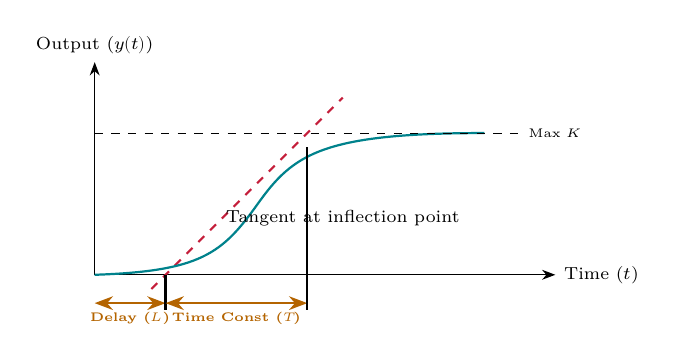
\begin{tikzpicture}[scale=0.9, transform shape]
  % Axes
  \draw[-Stealth, thin] (0,0) -- (6.5,0) node[right, font=\scriptsize] {Time ($t$)};
  \draw[-Stealth, thin] (0,0) -- (0,3.0) node[above, font=\scriptsize] {Output ($y(t)$)};
  
  % Tangent line
  \draw[dashed, color=myred, thick] (0.8, -0.2) -- (3.5, 2.5);
  
  % S-curve
  \draw[thick, color=myteal] (0,0) .. controls (1.5,0.05) and (1.8,0.3) .. (2.3,1.0) .. controls (2.8,1.7) and (3.2,2.0) .. (5.5,2.0);
  \draw[dashed] (0,2.0) -- (6.0,2.0) node[right, font=\tiny] {Max $K$};
  
  % Mark L and T
  \draw[Stealth-Stealth, thick, color=myamber] (0, -0.4) -- (1.0, -0.4) node[midway, below, font=\tiny\bfseries] {Delay ($L$)};
  \draw[thick] (1.0, 0) -- (1.0, -0.5);
  
  \draw[Stealth-Stealth, thick, color=myamber] (1.0, -0.4) -- (3.0, -0.4) node[midway, below, font=\tiny\bfseries] {Time Const ($T$)};
  \draw[thick] (3.0, 1.8) -- (3.0, -0.5);
  
  \node[font=\scriptsize] at (3.5, 0.8) {Tangent at inflection point};
\end{tikzpicture}
\end{tcolorbox}

Let $K$ be the process static gain. The transfer function model is $G(s) = \frac{K e^{-Ls}}{1 + sT}$.
\textbf{Tuning Parameters:}
  \begin{center}
  \small
  \begin{tabularx}{0.85\linewidth}{|B{3.0cm}|Y|Y|Y|}
  \hline
  \textbf{Controller Type} & $K_p$ & $T_i$ & $T_d$ \\ \hline
  \textbf{P} & $T / (KL)$ & $\infty$ & $0$ \\ \hline
  \textbf{PI} & $0.9\,T / (KL)$ & $3.3\,L$ & $0$ \\ \hline
  \textbf{PID} & $1.2\,T / (KL)$ & $2.0\,L$ & $0.5\,L$ \\ \hline
  \end{tabularx}
  \end{center}

\subsection{2. Ziegler-Nichols (ZN) Second Method (Closed-Loop)}
A closed-loop tuning method that increases proportional gain until the loop enters sustained, constant-amplitude oscillations.
\begin{enumerate}[label=\textbf{\arabic*.}, leftmargin=*]
  \item Turn off integral and derivative actions ($T_i = \infty, T_d = 0$).
  \item Increase $K_p$ slowly until the process output oscillates continuously. The gain at this point is the \textbf{Ultimate Gain ($K_u$)}, and the oscillation period is the \textbf{Ultimate Period ($P_u$)}.
\end{enumerate}

\textbf{Tuning Parameters:}
  \begin{center}
  \small
  \begin{tabularx}{0.85\linewidth}{|B{3.0cm}|Y|Y|Y|}
  \hline
  \textbf{Controller Type} & $K_p$ & $T_i$ & $T_d$ \\ \hline
  \textbf{P} & $0.5\,K_u$ & $\infty$ & $0$ \\ \hline
  \textbf{PI} & $0.45\,K_u$ & $0.83\,P_u$ & $0$ \\ \hline
  \textbf{PID} & $0.6\,K_u$ & $0.5\,P_u$ & $0.125\,P_u$ \\ \hline
  \end{tabularx}
  \end{center}

\subsection{3. Cohen-Coon Tuning Method}
Cohen-Coon tuning is designed for systems with a first-order plus dead time (FOPDT) response. Unlike ZN, it provides tuning rules that compensate for processes with large dead times (high ratio of delay $L$ to time constant $T$).
Let $K$ be the static gain, $\tau$ the time constant, and $\theta$ the dead time.
\textbf{Tuning Equations:}
  \begin{itemize}[leftmargin=*, itemsep=3.5pt]
    \item \textbf{PI Controller:}
      \[
      K_p = \frac{\tau}{K\theta} \left( 0.9 + \frac{\theta}{12\tau} \right), \qquad T_i = \theta \frac{30 + 3\theta/\tau}{9 + 20\theta/\tau}
      \]
    \item \textbf{PID Controller:}
      \[
      K_p = \frac{\tau}{K\theta} \left( 1.35 + \frac{\theta}{6\tau} \right), \quad T_i = \theta \frac{32 + 6\theta/\tau}{13 + 8\theta/\tau}, \quad T_d = \theta \frac{4}{11 + 2\theta/\tau}
      \]
  \end{itemize}

% ===============================================================================
\section{Implementation of PID Controllers}
% ===============================================================================

\subsection{1. Analog PID Implementation (Op-Amps)}
Analog controllers use operational amplifiers with capacitors and resistors in parallel branches to implement summing, integrating, and differentiating operations.

\begin{tcolorbox}[tikzbox, title={Analog Op-Amp Parallel PID Controller Circuit}]
\centering
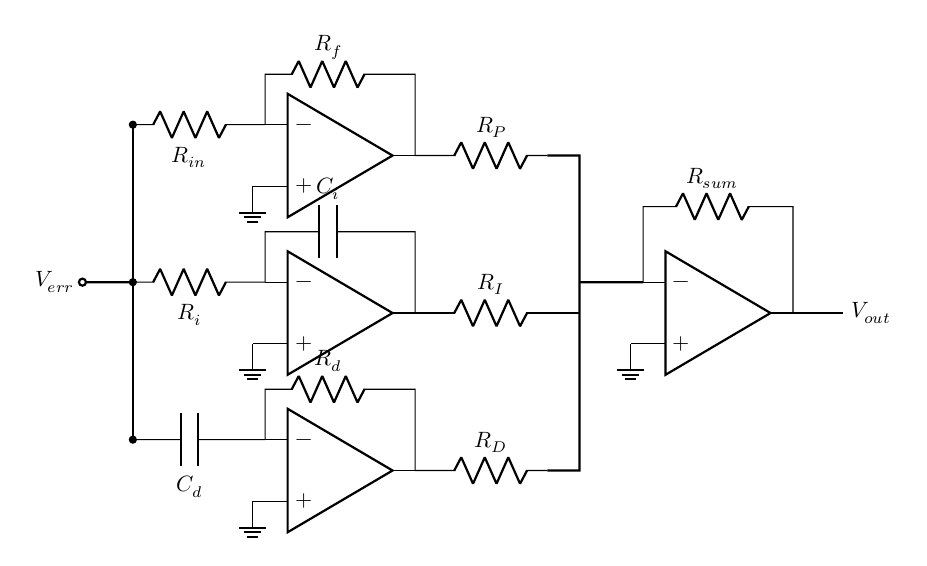
\begin{tikzpicture}[scale=0.8, transform shape]
  % Op-amps aligned at x=0
  \node[op amp] (op1) at (0, 2.5) {};
  \node[op amp] (op2) at (0, 0) {};
  \node[op amp] (op3) at (0, -2.5) {};
  
  % Summing Op-amp (A4)
  \node[op amp] (op4) at (6, 0) {};

  % Proportional Path (A1)
  \draw (op1.+) -- ++(-0.2, 0) node[ground] {};
  \draw (op1.-) -- ++(-0.3, 0) to[R, l=$R_{in}$, -*] ++(-1.8, 0) coordinate (p_in);
  \draw (op1.-) -- ++(0, 0.8) to[R, l=$R_f$] ++(2.0, 0) -| (op1.out);
  \draw (op1.out) -- ++(0.3, 0) to[R, l=$R_P$] ++(1.8, 0) coordinate (p_out);

  % Integral Path (A2)
  \draw (op2.+) -- ++(-0.2, 0) node[ground] {};
  \draw (op2.-) -- ++(-0.3, 0) to[R, l=$R_i$, -*] ++(-1.8, 0) coordinate (i_in);
  \draw (op2.-) -- ++(0, 0.8) to[C, l=$C_i$] ++(2.0, 0) -| (op2.out);
  \draw (op2.out) -- ++(0.3, 0) to[R, l=$R_I$] ++(1.8, 0) coordinate (i_out);

  % Derivative Path (A3)
  \draw (op3.+) -- ++(-0.2, 0) node[ground] {};
  \draw (op3.-) -- ++(-0.3, 0) to[C, l=$C_d$, -*] ++(-1.8, 0) coordinate (d_in);
  \draw (op3.-) -- ++(0, 0.8) to[R, l=$R_d$] ++(2.0, 0) -| (op3.out);
  \draw (op3.out) -- ++(0.3, 0) to[R, l=$R_D$] ++(1.8, 0) coordinate (d_out);

  % Bus lines on input side
  \draw[thick] (p_in) -- (d_in);
  \draw[thick] (i_in) to[short, -o] ++(-0.8, 0) node[left] {$V_{err}$};

  % Summing bus on output side
  \draw[thick] (p_out) -- (3.8, 2.5) -- (3.8, -2.5) -- (d_out);
  \draw[thick] (i_out) -- (3.8, 0);
  \draw[thick] (3.8, 0.49) -- (op4.-);

  % Summing Amplifier feedback & output
  \draw (op4.+) -- ++(-0.2, 0) node[ground] {};
  \draw (op4.-) -- ++(0, 1.2) to[R, l=$R_{sum}$] ++(2.2, 0) -| (op4.out);
  \draw (op4.out) -- ++(0.8, 0) node[right] {$V_{out}$};
\end{tikzpicture}
\end{tcolorbox}

\subsection{2. Digital PID Algorithms}
Digital controllers (PLCs, microcontrollers) run algorithms in discrete time steps $T_s$.

\begin{itemize}[leftmargin=*, itemsep=2.5pt]
  \item \textbf{Positional Algorithm:} Computes the absolute control output value $u(n)$ at step $n$:
  \begin{tcolorbox}[formulabox, title={\textbf{Positional Digital PID}}]
  \[
  u(n) = K_p e(n) + K_p \frac{T_s}{T_i} \sum_{k=0}^n e(k) + K_p \frac{T_d}{T_s} \big( e(n) - e(n-1) \big)
  \]
  \end{tcolorbox}
  \textit{Disadvantage:} Requires keeping track of the sum of all past errors, making it prone to integral windup.
  
  \item \textbf{Velocity (Incremental) Algorithm:} Computes only the \textit{change} in output $\Delta u(n) = u(n) - u(n-1)$ to be applied to the actuator (e.g. stepping a control valve motor):
  \begin{tcolorbox}[formulabox, title={\textbf{Velocity Digital PID}}]
  \[
  \Delta u(n) = K_p \big( e(n) - e(n-1) \big) + K_p \frac{T_s}{T_i} e(n) + K_p \frac{T_d}{T_s} \big( e(n) - 2e(n-1) + e(n-2) \big)
  \]
  \end{tcolorbox}
  \textit{Advantages:}
  \begin{enumerate}[label=\textbf{\arabic*.}, leftmargin=*]
    \item \textbf{No Integral Windup:} The summation term is absent, removing cumulative winding.
    \item \textbf{Shock-free Transfer:} If the controller is switched from Manual to Auto mode, there are no sudden output jumps because the output is updated incrementally.
  \end{enumerate}
\end{itemize}

\newpage

% ===============================================================================
% QUICK REVISION PAGE
% ===============================================================================
\begin{center}
  {\large\bfseries\color{myred} Quick Revision --- Module 3}\\[3pt]
  {\small\color{mydark} PID Tuning \& Control $|$ PE-EC802B}
\end{center}
\noindent{\color{myred}\rule{\linewidth}{1.2pt}}
\vspace{4pt}

\begin{tcolorbox}[formulabox, title={\textbf{Key Formulas at a Glance}}]
\renewcommand{\arraystretch}{1.35}
\begin{tabularx}{\linewidth}{B{5.2cm} X}
Continuous PID Equation & $u(t) = K_p \left( e(t) + \frac{1}{T_i} \int e\,dt + T_d \frac{de}{dt} \right)$ \\[4pt]
ZN 1st Method (PID tuning) & $K_p = 1.2 \frac{T}{KL}, \quad T_i = 2L, \quad T_d = 0.5L$ \\[4pt]
ZN 2nd Method (PID tuning) & $K_p = 0.6\,K_u, \quad T_i = 0.5\,P_u, \quad T_d = 0.125\,P_u$ \\[4pt]
Digital Positional PID & $u(n) = K_p \left[ e(n) + \frac{T_s}{T_i}\sum e(k) + \frac{T_d}{T_s}\Delta e(n) \right]$ \\[4pt]
Digital Velocity PID & $\Delta u(n) = K_p \Delta e(n) + K_p \frac{T_s}{T_i} e(n) + K_p \frac{T_d}{T_s} \Delta^2 e(n)$ \\
\end{tabularx}
\end{tcolorbox}

\begin{tcolorbox}[defbox, title={\textbf{One-Line Definitions}}]
\begin{itemize}[leftmargin=*, itemsep=2pt, topsep=0pt]
  \item \textbf{Proportional Band:} The range of input error required to drive the controller output through its full scale range ($PB = 100/K_p$).
  \item \textbf{Integral Windup:} Actuator saturation causing the integral term to build up excessively, leading to output overshoot.
  \item \textbf{Derivative Kick:} An output spike produced by derivative action responding to a sudden step change in setpoint.
  \item \textbf{Ultimate Gain ($K_u$):} The maximum gain in a P-only closed loop that causes constant-amplitude output oscillation.
  \item \textbf{FOPDT Model:} First-Order Plus Dead Time model representing static gain $K$, time constant $\tau$, and delay $\theta$.
\end{itemize}
\end{tcolorbox}

\begin{tcolorbox}[tikzbox, title={\textbf{Control Algorithm \& Tuning Method Comparisons}}]
\centering
\par\noindent
\renewcommand{\arraystretch}{1.3}
\begin{tabularx}{\linewidth}{|B{3.0cm}|Y|Y|}
\hline
\textbf{Property} & \textbf{Positional PID Algorithm} & \textbf{Velocity PID Algorithm} \\ \hline
\textbf{Output Type} & Computes actual control output $u(n)$ & Computes incremental change $\Delta u(n)$ \\ \hline
\textbf{Windup Risk} & High (requires mathematical clamping limits) & Low (inherently immune; no accumulator) \\ \hline
\textbf{Initialization} & Prone to bumps when switched Manual $\to$ Auto & Bumpless transfer is easy to implement \\ \hline
\textbf{Actuator Type} & Regular valves, voltage drives & Stepping valves, incremental drives \\ \hline
\end{tabularx}

\vspace{0.3cm}
\begin{tabularx}{\linewidth}{|B{3.0cm}|Y|Y|}
\hline
\textbf{Property} & \textbf{Ziegler-Nichols Tuning} & \textbf{Cohen-Coon Tuning} \\ \hline
\textbf{Dead Time Adapt} & Poor (cannot tune loops with delay $L > T/2$) & Good (incorporates $\theta/\tau$ ratio terms) \\ \hline
\textbf{Loop Behavior} & Damped response (quarter-amplitude decay) & Faster response with slightly larger overshoot \\ \hline
\textbf{Process State} & Open-loop (Method 1) or oscillating (Method 2) & Open-loop step test only \\ \hline
\end{tabularx}
\end{tcolorbox}

\begin{tcolorbox}[exambox, title={\textbf{Frequently Asked / Viva Questions}}]
\begin{enumerate}[leftmargin=*, itemsep=4pt]
  \item \Q{Why does a Proportional-only controller always exhibit a steady-state offset?}
    Consider a P controller output $u = K_p e + u_0$. For a constant disturbance, to maintain a non-zero control output ($u \ne u_0$), a non-zero error $e$ must exist. If the error $e$ became zero, the controller output would return to bias $u_0$, failing to counter the disturbance. Integral action is required to remove this offset.
  \item \Q{Explain the physical mechanism of Integral Windup and its mitigation.}
    If a large step change is applied, the controller saturates the actuator (e.g. valve 100\% open). The integral term continues integrating the remaining error, growing to a huge value. When the error changes sign, the valve cannot close until the integral term integrates down, causing overshoot. Mitigation: \textbf{anti-windup clamping} freezes the integrator once output saturates.
  \item \Q{How does "derivative-on-measurement" prevent derivative kick?}
    Setpoint step changes are instantaneous, creating an infinite derivative $de/dt$. Since process variables cannot change instantly due to physical inertia, the derivative of the process measurement $dy/dt$ remains finite. Taking the derivative of only the measurement terminal eliminates setpoint-step spikes.
  \item \Q{What are ultimate gain ($K_u$) and ultimate period ($P_u$) in ZN closed-loop tuning?}
    Ultimate gain $K_u$ is the proportional-only gain that drives the closed-loop system into sustained, constant-amplitude sinusoidal oscillations. The period of these sustained oscillations is the ultimate period $P_u$.
  \item \Q{What are the advantages of the digital velocity PID algorithm over the positional algorithm?}
    The velocity algorithm computes only the change in control output ($\Delta u$). It does not accumulate error, making it immune to integral windup. It is compatible with stepping motors and offers safe, bump-free switching between manual and automatic control modes.
  \item \Q{Under what process condition is Cohen-Coon tuning preferred over Ziegler-Nichols?}
    Cohen-Coon tuning is preferred when the process has a significant transport delay or dead time relative to its time constant ($\theta/\tau > 0.5$). Ziegler-Nichols tuning results in highly unstable loop control under large dead times.
\end{enumerate}
\end{tcolorbox}

\end{document}
